% !TeX program = xelatex
\documentclass[a4paper,10pt]{article}

% ============================================================================
% សន្លឹកកិច្ចការសិស្ស ស-ខ្មៅ (Student Guided-Inquiry Worksheet - Grade 8 ALG55)
% បរិបទ៖ ថ្នាក់រៀនគ្មានស្លាយ LCD – ៣.១ ពន្លាតការេនៃទ្វេធា និងផលគុណទ្វេធាឆ្លាស់សញ្ញា (២ ទំព័រ A4)
% ============================================================================
\usepackage[a4paper, left=0.90cm, right=0.90cm, top=0.75cm, bottom=0.85cm, footskip=0.45cm]{geometry}
\usepackage{amsmath, amssymb}
\usepackage{unicode-math}
\usepackage{fontspec}
\usepackage{array, colortbl}
\usepackage[table]{xcolor}
\usepackage{enumitem}
\usepackage{pifont}
\usepackage{fancyhdr}
\usepackage{lastpage}
\usepackage{tikz}
\usepackage[most]{tcolorbox}
\usetikzlibrary{calc, arrows.meta, positioning, babel}

\makeatletter
\let\@expl@@@mark@update@singlecol@structures@@\relax
\makeatother

\providecommand{\NGSFindFonts}{%
  \IfFileExists{C:/Windows/Fonts/cambria.ttc}{%
    \def\NGSSysPath{C:/Windows/Fonts/}%
    \def\NGSUserPath{C:/Users/KIT/AppData/Local/Microsoft/Windows/Fonts/}%
  }{%
    \IfFileExists{./fonts/KhmerOSsiemreap.ttf}{\def\NGSSysPath{./fonts/}\def\NGSUserPath{./fonts/}}{%
    \IfFileExists{../fonts/KhmerOSsiemreap.ttf}{\def\NGSSysPath{../fonts/}\def\NGSUserPath{../fonts/}}{%
    \IfFileExists{../../fonts/KhmerOSsiemreap.ttf}{\def\NGSSysPath{../../fonts/}\def\NGSUserPath{../../fonts/}}{%
    \IfFileExists{../../../fonts/KhmerOSsiemreap.ttf}{\def\NGSSysPath{../../../fonts/}\def\NGSUserPath{../../../fonts/}}{%
    \IfFileExists{../../../../fonts/KhmerOSsiemreap.ttf}{\def\NGSSysPath{../../../../fonts/}\def\NGSUserPath{../../../../fonts/}}{%
    \IfFileExists{../../../../../fonts/KhmerOSsiemreap.ttf}{\def\NGSSysPath{../../../../../fonts/}\def\NGSUserPath{../../../../../fonts/}}{%
    \IfFileExists{../../../../../../fonts/KhmerOSsiemreap.ttf}{\def\NGSSysPath{../../../../../../fonts/}\def\NGSUserPath{../../../../../../fonts/}}{%
      \def\NGSSysPath{../../../../../../../fonts/}\def\NGSUserPath{../../../../../../../fonts/}%
    }}}}}}}%
  }%
}
\NGSFindFonts

\setmathfont[Path={\NGSSysPath}, FontIndex=1, Scale=1.02]{cambria.ttc}
\defaultfontfeatures{Ligatures=TeX}

\setmainfont[
  Path={\NGSUserPath},
  Extension=.ttf,
  Script=Khmer,
  BoldFont={KhmerOSsiemreap},
  BoldFeatures={FakeBold=1.8},
  ItalicFont={KhmerOSsiemreap},
  ItalicFeatures={FakeSlant=0.25},
  BoldItalicFont={KhmerOSsiemreap},
  BoldItalicFeatures={FakeBold=1.8, FakeSlant=0.25}
]{KhmerOSsiemreap}

\newfontfamily\muol[Path={\NGSUserPath}, Extension=.ttf, Script=Khmer]{KhmerOSmuollight}
\newfontfamily\TimesEn[Path={\NGSSysPath}, Extension=.ttf, BoldFont={timesbd}, ItalicFont={timesi}, BoldItalicFont={timesbi}]{times}

\XeTeXlinebreaklocale "km"
\XeTeXlinebreakskip = 0pt plus 1pt minus 0.1pt

\definecolor{panelgray}{gray}{0.94}
\definecolor{headgray}{gray}{0.86}

\pagestyle{fancy}
\fancyhf{}
\renewcommand{\headrulewidth}{0pt}
\fancyfoot[L]{\fontsize{8pt}{10pt}\selectfont អនុវិទ្យាល័យព្រះក្រសាំង \en{|} គណិតវិទ្យា ថ្នាក់ទី៨ \en{|} មេរៀនទី៥ (៣.១ ពន្លាតការេនៃទ្វេធា និងផលគុណទ្វេធាឆ្លាស់សញ្ញា)}
\fancyfoot[R]{\fontsize{8.2pt}{10pt}\selectfont ទំព័រ \en{\thepage\ / \pageref{LastPage}}}

\setlength{\parindent}{0pt}
\setlength{\parskip}{0pt}
\setlength{\tabcolsep}{4pt}

\newcommand{\en}[1]{{\TimesEn #1}}
\newcommand{\enbf}[1]{{\TimesEn\textbf{#1}}}
\newcommand{\unit}[1]{\,\text{\en{#1}}}
\newcommand{\cnum}[1]{{\fontsize{10pt}{12pt}\selectfont\ding{\numexpr171+#1\relax}}}
\newcommand{\chk}{\tikz[baseline=-0.15ex]\draw[black, line width=0.8pt] (0,0) rectangle (0.25cm,0.25cm);}
\newcommand{\dotline}[1]{\makebox[#1]{\dotfill}}

\newcolumntype{L}[1]{>{\raggedright\arraybackslash}p{#1}}
\newcolumntype{C}[1]{>{\centering\arraybackslash}p{#1}}

\newcommand{\secbar}[2]{%
  \vspace{3pt}
  \noindent\colorbox{headgray}{\parbox{\dimexpr\linewidth-2\fboxsep\relax}{%
    \vspace{1.5pt}{\muol\fontsize{9.5pt}{13.5pt}\selectfont #1}\hfill{\fontsize{8.5pt}{12pt}\selectfont\textbf{#2}}\vspace{1.5pt}%
  }}\par\vspace{3pt}
}

\begin{document}
\fontsize{9.5pt}{14.2pt}\selectfont

% ============================================================================
% ទំព័រទី១៖ ក្បាលសន្លឹកកិច្ចការ + E1 + E2 + E3
% ============================================================================
\begin{tcolorbox}[enhanced, sharp corners, colback=white, colframe=black, boxrule=1.0pt, top=4pt, bottom=4pt, left=6pt, right=6pt]
  \begin{center}
    {\muol\fontsize{10.5pt}{15pt}\selectfont សន្លឹកកិច្ចការសិស្ស — មេរៀនទី៥៖ កន្សោមពីជគណិត \enbf{(}៣.១ សមភាពសំខាន់ៗ\enbf{)}}\\[2pt]
    {\footnotesize សៀវភៅសិក្សាគោលថ្នាក់ទី៨ ទំព័រ ៦៣--៦៦ \en{|} ការបំបែកផ្ទៃក្រឡាធរណីមាត្រ និងល្បិចគិតមាត់រហ័ស (គ្មានស្លាយ \en{LCD})}
  \end{center}
  \vspace{2pt}
  \hrule height 0.5pt
  \vspace{4pt}
  ឈ្មោះសិស្ស៖ \dotline{5.3cm} ថ្នាក់៖ \dotline{2.0cm} ដៃគូទី៖ \dotline{2.0cm} កាលបរិច្ឆេទ៖ \dotline{3.3cm}
\end{tcolorbox}

% -------------------- ផ្នែកទី១៖ E1 ENGAGE --------------------
\secbar{ផ្នែកទី១ ៖ បេសកកម្មភ្ជាប់បញ្ហា \enbf{(E1 — Engage)} — អន្ទាក់បាត់តួកណ្ដាល និងល្បិចគិតមាត់}{\en{3} នាទី (ទស្សន៍ទាយមុនរៀន)}

\begin{tcolorbox}[enhanced, sharp corners, colback=panelgray, colframe=black, boxrule=0.8pt, top=3.5pt, bottom=3.5pt, left=6pt, right=6pt]
  \begin{minipage}[c]{13.5cm}
    សិស្សម្នាក់សរសេរថា $(a + b)^2 = a^2 + b^2$ ។ បើយើងជំនួស $a=3,\; b=2$ គេបាន $(3+2)^2 = 5^2 = \dotline{1.2cm}$ ខណៈ $3^2 + 2^2 = 9 + 4 = \dotline{1.2cm}$ (ខុសគ្នាដល់ទៅ $\dotline{1.2cm}$)!\\[2pt]
    \textbf{ទស្សន៍ទាយមុនរៀន៖} តាមរូបការេជ្រុង $(a+b)$ ខាងស្ដាំ តើពន្លាតត្រឹមត្រូវនៃ $(a+b)^2$ គឺមួយណា?\\[1.5pt]
    \hspace*{0.3cm}\chk\ $a^2 + b^2$ \qquad\quad
    \chk\ $a^2 + ab + b^2$ \qquad\quad
    \chk\ $a^2 + 2ab + b^2$
  \end{minipage}\hfill
  \begin{minipage}[c]{4.7cm}
    \centering
    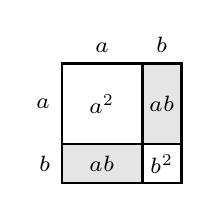
\begin{tikzpicture}[scale=0.66, every node/.style={font=\footnotesize, text=black}]
      \draw[black, line width=0.9pt, fill=white] (0,0.75) rectangle (1.55,2.30);
      \draw[black, line width=0.9pt, fill=gray!20] (1.55,0.75) rectangle (2.30,2.30);
      \draw[black, line width=0.9pt, fill=gray!20] (0,0) rectangle (1.55,0.75);
      \draw[black, line width=0.9pt, fill=white] (1.55,0) rectangle (2.30,0.75);
      \node at (0.775,1.525) {$a^2$};
      \node at (1.925,1.525) {$ab$};
      \node at (0.775,0.375) {$ab$};
      \node at (1.925,0.375) {$b^2$};
      \node[above=0.5pt] at (0.775,2.30) {$a$};
      \node[above=0.5pt] at (1.925,2.30) {$b$};
      \node[left=0.5pt] at (0,1.525) {$a$};
      \node[left=0.5pt] at (0,0.375) {$b$};
    \end{tikzpicture}
  \end{minipage}
\end{tcolorbox}

% -------------------- ផ្នែកទី២៖ E2 EXPLORE --------------------
\secbar{ផ្នែកទី២ ៖ រុករកសមភាពសំខាន់ៗទាំង ៣ \enbf{(E2 — Explore)}}{\en{11} នាទី (ពិភាក្សាដៃគូ)}

\textbf{ក. សកម្មភាពទី១ (រុករកការេនៃផលបូក ទំ.៦៣ និងការេនៃផលដក ទំ.៦៤)៖}
\begin{enumerate}[label=\arabic*., leftmargin=0.55cm, itemsep=4pt, topsep=2pt]
  \item \textbf{ការេនៃផលបូក $(a+b)^2$៖} បូកផ្ទៃក្រឡាទាំង ៤ បំណែក ឬពន្លាតតាមពិជគណិត៖\\
  $(a + b)^2 = (a + b)(a + b) = a^2 + ab + \dotline{1.2cm} + b^2 = \dotline{3.6cm}$ \quad \textbf{រូបមន្ត \en{(1)}} ។
  \item \textbf{ការេនៃផលដក $(a-b)^2$៖} ពន្លាតដោយប្រយ័ត្នសញ្ញា $(-b)\times(-b)$ នៅតួចុងក្រោយ៖\\
  $(a - b)^2 = (a - b)(a - b) = a^2 - ab - \dotline{1.2cm} + (-b)^2 = \dotline{3.6cm}$ \quad \textbf{រូបមន្ត \en{(2)}} ។
  \item \textbf{ផ្ទៀងផ្ទាត់ដោយលេខ៖} ចំពោះ $a=5,\; b=2$៖ $(5-2)^2 = 3^2 = \dotline{1.0cm}$ ហើយ $5^2 - 2(5)(2) + 2^2 = 25 - \dotline{1.1cm} + 4 = \dotline{1.1cm}$ ។ (បើច្រឡំដាក់ $-b^2$ នឹងបាន $25-20-4 = 1 \ne 9$!)
\end{enumerate}

\vspace{5pt}
\textbf{ខ. សកម្មភាពទី២ (រុករកផលគុណទ្វេធាឆ្លាស់សញ្ញា $(a-b)(a+b)$ និងផ្ទៃក្រឡាធរណីមាត្រ ទំ.៦៤--៦៥)៖}\par\vspace{3pt}
\begin{minipage}[c]{12.2cm}
  \begin{enumerate}[label=\arabic*., leftmargin=0.55cm, itemsep=4.5pt, topsep=1pt]
    \item \textbf{ពន្លាតតាមពិជគណិត៖} $(a - b)(a + b) = a^2 + ab - \dotline{1.2cm} - b^2 = \dotline{2.6cm}$ \textbf{\en{(3)}} ។
    \item \textbf{តាមផ្ទៃក្រឡា (ទំ.៦៥)៖} ការេធំដកការេតូចគឺ $a^2 - \dotline{1.0cm}$ ស្មើចតុកោណកែងទទឹង $(a-b)$ និងបណ្ដោយ $(a+\dotline{0.9cm})$ ។
    \item \textbf{សង្កេតចំនួនតួ៖} $(a\pm b)^2$ មាន \textbf{៣ តួ} ខណៈ $(a-b)(a+b)$ សល់តែ \textbf{២ តួ} ព្រោះតួកណ្ដាល $+ab$ និង $-ab$ \dotline{4.5cm} ។
    \item \textbf{សាកល្បងគិតមាត់៖} $101\times 99 = (100+1)(100-1) = 100^2 - 1^2 = \dotline{2.4cm}$ ។
  \end{enumerate}
\end{minipage}\hfill
\begin{minipage}[c]{6.2cm}
  \centering
  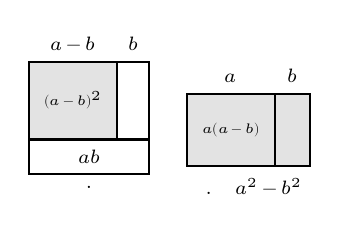
\begin{tikzpicture}[scale=0.68, every node/.style={font=\scriptsize, text=black}]
    \begin{scope}[shift={(0,0)}]
      \draw[black, line width=0.85pt, fill=gray!22] (0,0.65) rectangle (1.65,2.10);
      \draw[black, line width=0.85pt, fill=white] (1.65,0.65) rectangle (2.25,2.10);
      \draw[black, line width=0.85pt, fill=white] (0,0) rectangle (2.25,0.65);
      \node[font=\tiny] at (0.825,1.375) {$(a-b)^2$};
      \node at (1.125,0.325) {$ab$};
      \node[above=0.5pt] at (0.825,2.10) {$a-b$};
      \node[above=0.5pt] at (1.95,2.10) {$b$};
      \node[below=1pt] at (1.125,0) {ទំ.៦៤};
    \end{scope}
    \begin{scope}[shift={(2.95,0.15)}]
      \draw[black, line width=0.85pt, fill=gray!22] (0,0) rectangle (1.65,1.35);
      \draw[black, line width=0.85pt, fill=gray!22] (1.65,0) rectangle (2.30,1.35);
      \node[font=\tiny] at (0.825,0.675) {$a(a-b)$};
      \node[above=0.5pt] at (0.825,1.35) {$a$};
      \node[above=0.5pt] at (1.975,1.35) {$b$};
      \node[below=1pt] at (1.15,0) {ទំ.៦៥៖ $a^2-b^2$};
    \end{scope}
  \end{tikzpicture}
\end{minipage}

\vspace{5pt}
% -------------------- ផ្នែកទី៣៖ E3 EXPLAIN --------------------
\secbar{ផ្នែកទី៣ ៖ សង្ខេបរូបមន្តសមភាពសំខាន់ៗ និងធនាគារហេតុផល \enbf{(E3 — Explain)}}{\en{6} នាទី (កត់ត្រាខ្លឹមសារគោល)}

\begin{tcolorbox}[enhanced, sharp corners, colback=white, colframe=black, boxrule=0.85pt, top=5.5pt, bottom=5.5pt, left=6pt, right=6pt]
  \cnum{1} \textbf{ការេនៃផលបូក \en{(1)}៖} $(a + b)^2 = \dotline{4.0cm}$ \quad (មានសញ្ញា $+$ នៅមុខ $2ab$) ។\\[4.5pt]
  \cnum{2} \textbf{ការេនៃផលដក \en{(2)}៖} $(a - b)^2 = \dotline{4.0cm}$ \quad (មានសញ្ញា $-$ នៅមុខ $2ab$ តែតួចុងក្រោយគឺ $\mathbf{+b^2}$!) ។\\[4.5pt]
  \cnum{3} \textbf{ផលគុណទ្វេធាឆ្លាស់សញ្ញា \en{(3)}៖} $(a - b)(a + b) = \dotline{3.2cm}$ \quad (ផលដកនៃពីរការេ) ។\\[4.5pt]
  \cnum{4} \textbf{របាំងមេគុណ៖} ពេលតួមានមេគុណ ត្រូវលើកទាំងមេគុណជាការេ ឧ. $(2m)^2 = \dotline{1.5cm}$ និង $\left(\frac{1}{2}m\right)^2 = \dotline{1.5cm}$ ។\\[4.5pt]
  \cnum{5} \textbf{គិតមាត់រហ័ស៖} បំបែកលេខជិត $100$ ជា $(100 \pm k)^2$ ឬ $(100 + k)(100 - k)$ រួចជំនួសចូលសមភាព \en{(1)--(3)} ។\\[5.5pt]
  \centering
  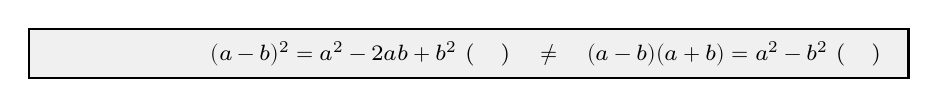
\begin{tikzpicture}
    \node[draw=black, line width=0.8pt, fill=panelgray, inner xsep=10pt, inner ysep=4.5pt, font=\footnotesize] {ប្រៀបធៀបកុំឱ្យច្រឡំ៖ \quad $(a - b)^2 = a^2 - 2ab + b^2$ (៣ តួ) \quad $\ne$ \quad $(a - b)(a + b) = a^2 - b^2$ (២ តួ)};
  \end{tikzpicture}
\end{tcolorbox}

\newpage
% ============================================================================
% ទំព័រទី២៖ E4 (លំហាត់គំរូ ទំ.៦៣-៦៦) + E5 (ប្រតិបត្តិ + Exit Check) + កិច្ចការផ្ទះ
% ============================================================================

% -------------------- ផ្នែកទី៤៖ E4 ELABORATE --------------------
\secbar{ផ្នែកទី៤ ៖ អនុវត្តលំហាត់គំរូ និងកំសាន្តគណិតវិទ្យា \enbf{(E4 — Elaborate)}}{\en{10} នាទី (បំពេញតាមគំរូ)}

\textbf{១. លំហាត់គំរូពន្លាតកន្សោមពីជគណិត (សៀវភៅគោល ទំ.៦៣--៦៥)៖}
\begin{itemize}[leftmargin=0.5cm, itemsep=3.5pt, topsep=2pt]
  \item \textbf{គំរូទី១ (ទំ.៦៣--៦៥)៖} $(x + 3)^2 = \dotline{3.5cm}$ \;;\; $(x - 1)^2 = \dotline{3.5cm}$ \;;\; $(x - 2)(x + 2) = \dotline{2.6cm}$ ។
  \item \textbf{គំរូទី២ (ទំ.៦៣)៖} $(2m + 3n)^2 = (2m)^2 + 2(2m)(3n) + (3n)^2 = \dotline{5.2cm}$ ។
  \item \textbf{គំរូទី២ (ទំ.៦៤)៖} $\left(\dfrac{1}{2}m - n\right)^2 = \left(\dfrac{1}{2}m\right)^2 - 2\left(\dfrac{1}{2}m\right)(n) + n^2 = \dotline{4.8cm}$ ។
  \item \textbf{គំរូទី២ (ទំ.៦៥)៖} $\left(\dfrac{1}{2}m - 3n\right)\left(\dfrac{1}{2}m + 3n\right) = \left(\dfrac{1}{2}m\right)^2 - (3n)^2 = \dotline{3.8cm}$ ។
\end{itemize}

\vspace{3pt}
\textbf{២. លំហាត់គំរូគិតលេខមាត់ (ទំ.៦៣--៦៥) និងកំសាន្តគណិតវិទ្យា (ទំ.៦៦)៖}
\begin{itemize}[leftmargin=0.5cm, itemsep=3.5pt, topsep=2pt]
  \item $101^2 = (100 + 1)^2 = 100^2 + 2(100)(1) + 1^2 = 10000 + \dotline{1.4cm} + 1 = \dotline{2.0cm}$ ។
  \item $99^2 = (100 - 1)^2 = 100^2 - 2(100)(1) + 1^2 = 10000 - \dotline{1.4cm} + 1 = \dotline{2.0cm}$ ។
  \item $101 \times 99 = (100 + 1)(100 - 1) = 100^2 - 1^2 = 10000 - 1 = \dotline{2.0cm}$ ។
  \item \textbf{កំសាន្តគណិតវិទ្យា (ទំ.៦៦)៖} $(1+1)(1-1)=0$ \;;\; $(2+1)(2-1)=3$ \;;\; $(3+2)(3-2)=5$ \;;\; $(4+3)(4-3)=\dotline{1.1cm}$ \;;\; $(10+9)(10-9)=\dotline{1.1cm}$ ។\\
  \textbf{ឆ្លុះបញ្ចាំង៖} សង្កេតឃើញថា $(n + (n-1))(n - (n-1)) = n^2 - (n-1)^2 = \dotline{2.8cm}$ (ស្មើផលបូកនៃចំនួនតគ្នាទាំងពីរ!) ។
\end{itemize}

% -------------------- ផ្នែកទី៥៖ E5 EVALUATE --------------------
\secbar{ផ្នែកទី៥ ៖ ហ្វឹកហាត់ «ប្រតិបត្តិ» និងតេស្តរហ័ស \enbf{(E5 — Evaluate)}}{\en{10} នាទី (ធ្វើដោយខ្លួនឯង រួចប្ដូរផ្ទៀង)}

\textbf{១. ប្រតិបត្តិពន្លាតការេនៃផលបូក (ទំ.៦៤) ការេនៃផលដក (ទំ.៦៥) និងទ្វេធាឆ្លាស់សញ្ញា៖}

\vspace{2pt}
{\renewcommand{\arraystretch}{1.44}
\begin{tabular}{|L{9.1cm}|L{9.1cm}|}
\hline
\cellcolor{headgray}\textbf{ប្រតិបត្តិ ទំ.៦៤ — រូបមន្ត $(a+b)^2$} & \cellcolor{headgray}\textbf{ប្រតិបត្តិ ទំ.៦៥ — រូបមន្ត $(a-b)^2$} \\
\hline
ក. $(b + 2a)^2 = \dotline{5.6cm}$ & ក. $(x - 2y)^2 = \dotline{5.6cm}$ \\
\hline
ខ. $(5x + 2y)^2 = \dotline{5.5cm}$ & ខ. $(5b - y)^2 = \dotline{5.6cm}$ \\
\hline
គ. $(6x^2 + 4)^2 = \dotline{5.4cm}$ & គ. $(x - 4y)^2 = \dotline{5.6cm}$ \\
\hline
ឃ. $(a + 5)^2 = \dotline{5.7cm}$ & ឃ. $\left(\dfrac{1}{5}a - 5\right)^2 = \dotline{5.2cm}$ \\
\hline
\cellcolor{panelgray}អនុវត្ត \en{(3)}៖ $(3x - 5)(3x + 5) = \dotline{3.8cm}$ & \cellcolor{panelgray}អនុវត្ត \en{(3)}៖ $(5 + 4)(5 - 4) = \dotline{3.8cm}$ \\
\hline
\end{tabular}}

\vspace{4pt}
\begin{tcolorbox}[enhanced, sharp corners, colback=panelgray, colframe=black, boxrule=0.85pt, top=3pt, bottom=3pt, left=6pt, right=6pt]
  \textbf{២. បិទបេសកកម្ម \en{E1} និងតេស្តរហ័ស (\en{Exit Check — 60} វិនាទី)៖}\\[2pt]
  $\bullet$ \textbf{ចម្លើយបេសកកម្ម \en{E1}៖} $(a+b)^2 \ne a^2+b^2$ ព្រោះមានតួកណ្ដាល $\dotline{1.8cm}$ ហើយ $101\times 99 = \dotline{1.8cm}$ ។\\[2pt]
  $\bullet$ \textbf{សំណួរតេស្តរហ័ស៖} តើពន្លាតនៃ $(3x - 4y)^2$ ស្មើនឹងកន្សោមមួយណា? (គូសរង្វង់ជម្រើសត្រឹមត្រូវ)\\[1.5pt]
  \hspace*{0.3cm}\enbf{A.}\; $9x^2 - 16y^2$ \qquad
  \enbf{B.}\; $9x^2 - 12xy + 16y^2$ \qquad
  \enbf{C.}\; $9x^2 - 24xy + 16y^2$ \qquad
  \enbf{D.}\; $9x^2 - 24xy - 16y^2$
\end{tcolorbox}

% -------------------- ផ្នែកទី៦៖ កិច្ចការផ្ទះ --------------------
\secbar{ផ្នែកទី៦ ៖ ប័ណ្ណកិច្ចការផ្ទះ \enbf{(Homework)} និងការអានជាមុន}{សៀវភៅសិក្សាគោល ទំ.៧៣}

\begin{tcolorbox}[enhanced, sharp corners, colback=white, colframe=black, boxrule=0.8pt, borderline={0.6pt}{2pt}{dashed}, top=3pt, bottom=3pt, left=6pt, right=6pt]
  \textbf{១. លំហាត់ទី៨ ក (ទំ.៧៣)៖} ស្រាយបញ្ជាក់សមភាព $(1 + x)(1 - x)(1 + x^2) = 1 - x^4$ ។\\[1.5pt]
  \textbf{២. លំហាត់ទី៩ (ទំ.៧៣)៖} មុធាគណនាដោយប្រើសមភាពសំខាន់ៗ៖ $39\times 41,\; 54\times 66,\; 19\times 21,\; 39^2,\; 102^2 - 101^2,\; 54^2 - 46^2$ ។\\[1.5pt]
  \textbf{៣. លំហាត់ទី១០ គ--ឃ (ទំ.៧៣)៖} ពន្លាត និងបង្រួម៖ គ) $(a - 3b)^2 + 9(a^2 - 3b) + 5$ \;;\; ឃ) $-x(4x - 3y) + x^2 - 12xy$ ។\\[1.5pt]
  $\bullet$ \textbf{អានជាមុន៖} ចំណុច \textbf{៣.២ ពន្លាតគូបនៃទ្វេធា និងត្រីកោណប៉ាស្កាល់} (សៀវភៅគោល ទំព័រ ៦៦--៦៨) ។
\end{tcolorbox}

\end{document}
